\sect{7.3\quad 拟阵复形}
若 $M=M(S)$ 是有限集 $S$ 上秩为 $r$ 的拟阵，其全部独立集构成 $(r-1)$ 维单纯复形，记为 $\IN(M)$，称为\textbf{拟阵复形}。拟阵复形是纯的是拟阵理论的基本事实；我们很快将看到它也可壳。事实上，拟阵复形既可用纯性刻画，也可用可壳性刻画（习题7.3.1和定理7.3.4）。
给底层点集一个线性次序，会揭示拟阵的一些重要性质，而这些性质本身不依赖次序。\textbf{有序拟阵} $M(S,\omega)$ 指拟阵 $M(S)$ 连同 $S$ 上的线性次序 $\omega$。约定将 $k$ 元子集按 $x_1<\cdots<x_k$ 写为 $[x_1,\ldots,x_k]$。其\textbf{字典序}定义为：若某个位置 $e$ 满足 $x_i=y_i$（$i<e$）且 $x_e<y_e$，则 $[x_1,\ldots,x_k]$ 排在 $[y_1,\ldots,y_k]$ 之前。下文比较基时均使用此诱导次序。
回忆：若 $B$ 是基且 $p\in S-B$，则 $B\cup p$ 含唯一回路 $\ci(B,p)$；对偶地，若 $b\in B$，则 $(S-B)\cup b$ 含唯一余回路（bond）$\bo(B,b)$。基本回路和基本余回路满足：
\st{引理7.3.1}$b\in\ci(B,p)\Longleftrightarrow(B-b)\cup p\text{ 是基}\Longleftrightarrow p\in\bo(B,b)$。
设 $C$ 是有序拟阵的回路，$c$ 是其中最小元素，则 $C-c$ 称为\textbf{断路}。不含任何断路的基称为\textbf{nbc基}。这个概念在后续各节十分重要；这里先在下面的技术引理中使用，它是本节和下一节的关键。
\st{引理7.3.2}设 $M(S,\omega)$ 是有序拟阵，基 $B$ 在字典序中先于基 $C$。则存在也先于 $C$ 的基 $A$，使 $B\cap C\subseteq A\cap C$ 且 $|A\cap C|=|C|-1$。此外，若 $C$ 是nbc基，可选择 $A$ 也是nbc基。
\pr 设 $B=[b_1,\ldots,b_r]$、$C=[c_1,\ldots,c_r]$，且 $b_i=c_i$（$i<e$）、$b_e\ne c_e$。则 $b_e<c_i$（$i=e,\ldots,r$）。由基交换性质，存在 $y\in C-B$，使 $A_1=(C-y)\cup b_e$ 为基。第一条结论可取 $A=A_1$。
\src{7}
对第二条，设 $C$ 是nbc基。若 $A_1$ 不是nbc基，则存在 $a_1\in S-A_1$，它是基本回路 $\ci(A_1,a_1)$ 的最小元素。$b_e$ 必属于此回路，否则 $C$ 将包含断路 $\ci(A_1,a_1)-a_1$。因此 $A_2=(A_1-b_e)\cup a_1$ 是基，且先于 $A_1$，满足 $B\cap C\subseteq A_2\cap C$、$|A_2\cap C|=r-1$。若 $A_2$ 仍不是nbc基，就重复此过程，有限步后得到所需的 $A=A_k$。\qed
去掉关于nbc基的最后一句，引理7.3.2等价于以下结果（比较(7.3)）：
\st{定理7.3.3}有序拟阵 $M(S,\omega)$ 的基的 $\omega$ 字典序是 $\IN(M)$ 的壳序。特别地，所有拟阵复形都可壳。
因此底集的每个线性次序都诱导壳序，这种丰富性实际上刻画了拟阵。
\st{定理7.3.4}单纯复形 $\Delta$ 是拟阵复形，当且仅当它纯，且顶点的每个排序都诱导壳序。
\pr 必要性即定理7.3.3。反之，设纯复形 $\Delta$ 不是拟阵复形。存在 $U\subseteq V$，使诱导子复形 $\Delta_U=\{F\in\Delta:F\subseteq U\}$ 不纯（习题7.3.1）。取其最小维刻面 $F$；在维数大于 $\dim F$ 的刻面中，取使 $|F\cap G|$ 尽可能大的 $G$。将顶点排为：$F-G$ 在前，$G$ 次之，其余在后。令 $\widetilde G$ 为首个包含 $G$ 的刻面，$\widetilde F$ 为任意包含 $F$ 的刻面。由极大性，$\widetilde F\cap U=F$，$\widetilde G\cap U=G$。所选次序保证：刻面 $H$ 先于 $\widetilde G$ 当且仅当 $H\cap(F-G)\ne\varnothing$。特别地，$\widetilde F$ 先于 $\widetilde G$。由于 $F,G$ 是 $\Delta_U$ 的刻面且 $|F|<|G|$，有 $|F\cap G|\le|G|-2$，故 $|\widetilde F\cap\widetilde G|\le|\widetilde G|-2$。
若有先于 $\widetilde G$ 的刻面 $H$ 和 $g\in\widetilde G$ 满足 $\widetilde F\cap\widetilde G\subseteq H\cap\widetilde G=\widetilde G-g$，则 $g\in\widetilde G-\widetilde F$，且 $H-\widetilde G=\{h\}$，$h\in F-G$。若 $g\in\widetilde G-G$，则 $G\cup h\subseteq H\cap U$，与 $G$ 极大矛盾。若 $g\in G-F$，则 $G'=(G-g)\cup h$ 是 $\Delta_U$ 中维数等于 $\dim G>\dim F$ 的面，且 $|F\cap G'|>|F\cap G|$，与 $G$ 的选择矛盾。因此无此 $H$，所诱导次序不是壳序。\qed
现在求壳多项式。若 $p\in S-B$ 是 $\ci(B,p)$ 的最小元素，称其在 $B$ 中\textbf{外活跃}，否则称外被动。对偶地，若 $p\in B$ 是 $\bo(B,p)$ 的最小元素，称其\textbf{内活跃}，否则称内被动。分别用 $\EA(B),\EP(B),\IA(B),\IP(B)$ 记这四类元素集。称 $i(B)=|\IA(B)|$ 为内活性，$e(B)=|\EA(B)|$ 为外活性。显然 $p$ 在 $B$ 中内活跃，当且仅当它在对偶有序拟阵 $M^*(S,\omega)$ 的基 $S-B$ 中外活跃。
\st{例7.3.5}设 $M$ 是图2(a)仿射空间中点线关系所定义的拟阵，也等价于图2(b)的图拟阵。
\src{8}
\begin{center}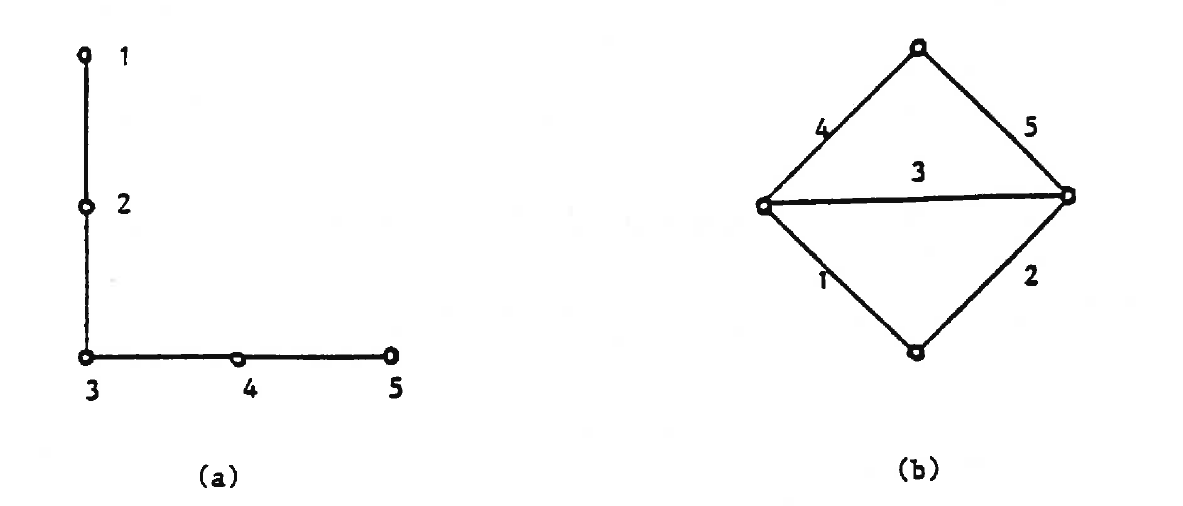
\includegraphics[width=.8\textwidth]{images/fig2.png}\par 图2\end{center}
将8个基按字典序列出，并标明各基的活跃元素：
\begin{center}\begin{tabular}{ccc}\toprule 基&内活跃元素&外活跃元素\\\midrule
$B_1=[1,2,4]$&$1,2,4$&无\\
$B_2=[1,2,5]$&$1,2$&无\\
$B_3=[1,3,4]$&$1,4$&无\\
$B_4=[1,3,5]$&$1$&无\\
$B_5=[1,4,5]$&$1$&$3$\\
$B_6=[2,3,4]$&$4$&$1$\\
$B_7=[2,3,5]$&无&$1$\\
$B_8=[2,4,5]$&无&$1,3$\\\bottomrule\end{tabular}\end{center}
$\IN(M)$ 的图像见图3：它是三角双锥的表面，加上内部两个三角形145和245。观察基序列 $B_1,\ldots,B_8$ 怎样给出壳序，颇有启发。
\begin{center}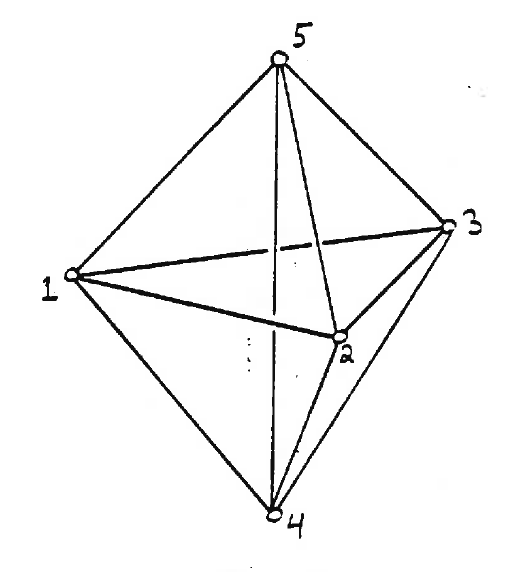
\includegraphics[width=.46\textwidth]{images/fig3.png}\par 图3\end{center}
\src{9}
再考虑有序拟阵基的字典序。由引理7.3.1，$B-b$ 包含于一个先于 $B$ 的基，当且仅当 $b$ 在 $B$ 中内被动。因此
\[\RR(B)=\IP(B).\tag{7.9}\]
所以拟阵复形 $\Delta=\IN(M)$ 的壳多项式为
\[h_\Delta(x)=\sum_Bx^{|B-\RR(B)|}=\sum_Bx^{|\IA(B)|}=\sum_Bx^{i(B)}.\tag{7.10}\]
对偶地，$\Delta^*=\IN(M^*)$ 的壳多项式为 $h_{\Delta^*}(y)=\sum_By^{e(B)}$。两处都对 $M$ 的全部基求和。因此很自然将二者合成二元多项式
\[T_M(x,y)=\sum_Bx^{i(B)}y^{e(B)}.\tag{7.11}\]
但有一个困难：我们由命题7.2.3知道
\[T_M(x,1)=h_{\IN(M)}(x),\qquad T_M(1,y)=h_{\IN(M^*)}(y)\tag{7.12}\]
与次序无关，却不能立即知道 $T_M(x,y)$ 本身与次序无关。下面将证明这一点，故称为 $M$ 的\textbf{Tutte多项式}的 $T_M$ 只依赖拟阵结构。
先回到例7.3.5。由活跃元素表得
\[\begin{aligned}
T_M(x,y)&=x^3+x^2+x^2+x+xy+xy+y+y^2\\
&=x^3+2x^2+y^2+2xy+x+y.
\end{aligned}\]
因此 $h_{\IN(M)}(x)=x^3+2x^2+3x+2$，而 $h_{\IN(M^*)}(y)=y^2+3y+4$。
\st{命题7.3.6}对有序拟阵 $M(S,\omega)$，每个基 $B$ 对应的区间 $[\IP(B),S-\EP(B)]$ 划分布尔代数 $2^S$。
\pr 需证明每个 $A\subseteq S$ 存在唯一基 $B_A$，使 $\IP(B_A)\subseteq A\subseteq S-\EP(B_A)$。
\src{10}
令 $X_A$ 是限制拟阵 $M_A$ 的字典序最大基。由命题7.2.2及(7.9)，存在唯一的 $M$ 的基 $B_A$，使 $\IP(B_A)\subseteq X_A\subseteq B_A$。取 $a\in A-B_A=A-X_A$，反设它在 $B_A$ 中外被动，则有 $b\in B_A$，使 $b<a$ 且 $(B_A-b)\cup a$ 是基。若 $b\notin A$，则 $X_A\cup a$ 独立，与 $X_A$ 是 $M_A$ 的基矛盾。若 $b\in A$，则 $b\in B_A\cap A=X_A$，且 $(X_A-b)\cup a$ 是字典序更大的基，仍矛盾。因此 $A-B_A$ 中所有元素都外活跃，从而 $\IP(B_A)\subseteq X_A\subseteq A\subseteq S-\EP(B_A)$。
再设某基 $B$ 满足 $\IP(B)\subseteq A\subseteq S-\EP(B)$。注意
\[\EA(B)\subseteq\operatorname{cl}(\IP(B)).\tag{7.13}\]
事实上，若 $p\in S-B$ 外活跃，令 $C=\ci(B,p)$，$C'=C-p$。对每个 $q\in C'$，$p<q$ 且 $(B-q)\cup p$ 为基，所以 $q$ 内被动。又 $p\in\operatorname{cl}(C')$，$C'\subseteq\IP(B)$，故(7.13)成立。这说明 $X=B\cap A$ 是 $M_A$ 的基。
若 $X\ne X_A$，写 $X=\{x_1<\cdots<x_a\}$、$X_A=\{y_1<\cdots<y_a\}$。由 $X_A$ 最大，存在 $e$ 使 $x_i=y_i$（$i<e$），且 $x_e<y_i$（$i\ge e$）。由基交换公理，某个 $j\ge e$ 使 $(X-x_e)\cup y_j$ 为基。于是 $y_j$ 在 $X$ 中外被动，因而在 $B$ 中也外被动，与 $A\subseteq S-\EP(B)$ 矛盾。因此 $X=X_A$，再由 $\IP(B)\subseteq X\subseteq B$ 得 $B=B_A$。\qed
\st{定理7.3.7}对有序拟阵 $M$，有
\[T_M(1+\xi,1+\eta)=\sum_{A\subseteq S}\xi^{r(S)-r(A)}\eta^{r^*(S)-r^*(S-A)},\]
其中 $r,r^*$ 分别为 $M,M^*$ 的秩函数。特别地，Tutte多项式与 $S$ 的次序无关。
\pr 若 $\IP(B)\subseteq A\subseteq S-\EP(B)$，(7.13)给出 $r(A)=|A\cap B|$，故 $r(S)-r(A)=|B-A|$；对偶地，$r^*(S)-r^*(S-A)=|(S-B)-(S-A)|=|A-B|$。由命题7.3.6，
\[\begin{aligned}
\sum_{A\subseteq S}\xi^{r(S)-r(A)}\eta^{r^*(S)-r^*(S-A)}
&=\sum_{B\text{ 为基}}\sum_{\IP(B)\subseteq A\subseteq S-\EP(B)}\xi^{|B-A|}\eta^{|A-B|}\\
&=\sum_B\sum_{j,k\ge0}\binom{i(B)}j\binom{e(B)}k\xi^j\eta^k\\
&=\sum_B(1+\xi)^{i(B)}(1+\eta)^{e(B)}=T_M(1+\xi,1+\eta).
\end{aligned}\]\qed
\src{11}
本卷第6章详细讨论Tutte多项式，更多内容可参阅那里。本节结束前指出，由(7.12)和推论7.2.4，$\chi(\IN(M))=(-1)^{r-1}T_M(0,1)$。命题7.4.7将给出另一表达式。
